% ============================================================
%  Experiment 6 --- Stepper Motor Control with FPGA
% ============================================================
\experimentheader{6}{Stepper Motor Control}{Stepper Motor Control with FPGA}{FPGA Lab}

\begin{objectives}
  \begin{enumerate}
    \item To design digital circuits in an FPGA to control a stepper motor.
    \item To use Verilog as a design entry method in Altera Quartus II Software.
    \item To simulate the circuit using Altera Quartus II Software.
    \item To download the design onto an Altera DE2 board.
  \end{enumerate}
\end{objectives}

\begin{equipment}
  \begin{itemize}
    \item Altera Quartus II software
    \item Altera DE2 board
    \item Parallax 4-phase, 12\,V, 75\,$\Omega$ unipolar stepper motor
    \item ULN2003 Darlington transistor array (motor driver)
  \end{itemize}
\end{equipment}

\begin{introduction}
  Unlike an ordinary DC motor, a stepper motor does not spin freely when power is applied --- it must be driven with a continuously pulsed sequence of specific coil-energising patterns. Each pulse advances the rotor by a fixed step angle (for this motor, $3.6^\circ$ per step), which is what gives stepper motors their positioning precision: as long as speed and torque stay within the motor's limits, the controller always knows the rotor's exact position.

  The rotor is driven by the interaction of magnetic fields as coils are switched on and off in sequence. Table~\ref{tab:exp6-stepseq} shows the normal four-coil unipolar step sequence; taking a step means driving two of the four coil-driver pins high at a time, in the order shown, through the ULN2003 driver.
\end{introduction}

\needspace{4cm}
\begin{boxedtable}
  \captionof{table}{Normal step sequence for a four-coil unipolar stepper motor.}
  \label{tab:exp6-stepseq}
  {\renewcommand{\arraystretch}{1.5}
    \centering
    \begin{tabular}{lccccc}
      \toprule
      Coil    & Step 1 & Step 2 & Step 3 & Step 4 & Step 1 \\
      \midrule
      1 (A)   & 1      & 1      & 0      & 0      & 1      \\
      2 (\=A) & 0      & 0      & 1      & 1      & 0      \\
      3 (B)   & 1      & 0      & 0      & 1      & 1      \\
      4 (\=B) & 0      & 1      & 1      & 0      & 0      \\
      \bottomrule
    \end{tabular}
  }
\end{boxedtable}
\newpage

\begin{procedure}

  \textbf{Activity 1 --- Verilog stepper motor controller}\vspace{2pt}

  \textit{Objective: write Verilog code to control the motion of a stepper motor.}

  \begin{enumerate}
    \item Open Quartus II and start the New Project Wizard.
          \begin{itemize}
            \item Working directory: \texttt{fpga}; project name: \texttt{activity1}; top-level entity: \texttt{step}.
            \item Device family: Cyclone II, device \texttt{EP2C35F672C6N}.
            \item Accept the default EDA tool settings and finish.
          \end{itemize}
    \item Create a new Verilog HDL file and enter the code in Listing~\ref{lst:exp6-step} (\texttt{step}, \texttt{divider}, and \texttt{stepper} modules).
    \item Save as \texttt{step} and start compilation.
    \item Use \textbf{Tools} $\to$ \textbf{Netlist Viewer} $\to$ \textbf{RTL Viewer} to generate the block overview shown in Figure~\ref{fig:exp6-rtl}.
    \item Assign pin numbers as shown in Table~\ref{tab:exp6-pins} (refer to the DE2 user manual). For the \texttt{phaseout} outputs that interface with the stepper motor driver, use expansion header \texttt{GPIO\_0}.
    \item Download the program to the Altera DE2 board.
    \item Discuss the result.
  \end{enumerate}

  \begin{boxedfigure}
    \centering
    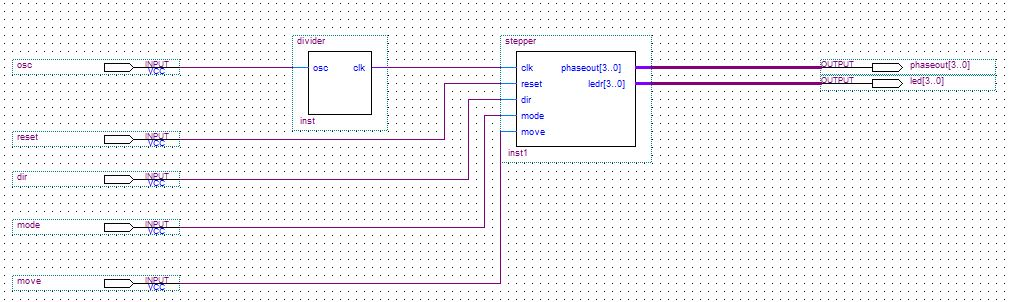
\includegraphics[width=\linewidth]{figures/Exp6_Figure_1.jpg}
    \captionof{figure}{RTL Viewer overview of the \texttt{step} top-level module.}
    \label{fig:exp6-rtl}
  \end{boxedfigure}

  \needspace{4cm}
  \begin{boxedtable}
    \captionof{table}{Pin assignment for stepper motor control.}
    \label{tab:exp6-pins}
    {\renewcommand{\arraystretch}{1.5}
      \centering
      \begin{tabular}{cccc}
        \toprule
        \# & Node name   & Direction & Pin location \\
        \midrule
        1  & osc         & Input     &              \\
           & dir (SW0)   & Input     &              \\
           & mode (SW1)  & Input     &              \\
           & move (SW2)  & Input     &              \\
           & reset (SW3) & Input     &              \\
        2  & ledr[3]     & Output    &              \\
        3  & ledr[2]     & Output    &              \\
        4  & ledr[1]     & Output    &              \\
        5  & ledr[0]     & Output    &              \\
        6  & phaseout[3] & Output    &              \\
        7  & phaseout[2] & Output    &              \\
        8  & phaseout[1] & Output    &              \\
        9  & phaseout[0] & Output    &              \\
        \bottomrule
      \end{tabular}
    }
  \end{boxedtable}

  \begin{codepanel}{step.v --- top-level module}{verilogstyle}
    \begin{lstlisting}
//============================================================
// Stepper Motor Controller
//============================================================
// TOP LEVEL MODULE
// reset (active low) brings the shaft to its reference position.
// mode selects step (1) or continuous (0) operation.
// dir selects clockwise (1) or anti-clockwise (0) motion.
// move shifts the shaft by one half-step in step mode.
module step(osc, reset, dir, mode, move, phaseout, ledr);
  input  osc, reset, mode, dir, move;
  output [3:0] phaseout, ledr;

  wire clk;

  divider d1 (
    .osc (osc),
    .clk (clk)
  );

  stepper s1 (
    .clk      (clk),
    .reset    (reset),
    .dir      (dir),
    .mode     (mode),
    .move     (move),
    .phaseout (phaseout)
  );
endmodule
\end{lstlisting}
  \end{codepanel}
  \vspace{-4pt}

  \begin{codepanel}{step.v --- motor controller module (part 1 of 2)}{verilogstyle}
    \begin{lstlisting}
// Module stepper is the motor controller.
module stepper(clk, reset, dir, mode, move, phaseout);
  input  clk, reset, dir, mode, move;
  output [3:0] phaseout;
  reg [3:0] phaseout, position, ledr;

  always @(posedge clk or negedge reset)
  begin
    if (reset == 0) begin
      // motor resets to phase 1000 when reset is asserted
      phaseout = 4'b1000;
      ledr     = phaseout;
    end
    else begin
      if (mode == 0) begin
        // Mode = 0: continuous motion.
        // The 8-state sequence below follows Table 1 in both
        // directions; only the first two states are shown here,
        // the remaining six states (0100, 0110, 0010, 0011,
        // 0001, 1001) follow the identical if(dir==0)/else
        // pattern, cycling back to 1000.
        case (phaseout)
          4'b1000: if (dir == 0) begin
            phaseout = 4'b1100;  ledr = phaseout;
          end else begin
            phaseout = 4'b1001;  ledr = phaseout;
          end
          4'b1100: if (dir == 0) begin
            phaseout = 4'b0100;  ledr = phaseout;
          end else begin
            phaseout = 4'b1000;  ledr = phaseout;
          end
          // ... 4'b0100, 4'b0110, 4'b0010, 4'b0011,
          //     4'b0001, 4'b1001 follow the same pattern ...
          default: $display("invalid input");
        endcase
      end
      else begin
        // Mode = 1: single-step motion, advances only when
        // move == 0. Uses the same 8-state sequence as above,
        // indexed by `position` instead of `phaseout`.
        if (move == 1'b0) begin
          case (position)
            // ... identical 8-state sequence as continuous
            //     mode, see Table 1 ...
            default: $display("invalid input");
          endcase
        end
      end
    end
  end
\end{lstlisting}
  \end{codepanel}
  \vspace{-4pt}

  \begin{codepanel}{step.v --- motor controller module (part 2 of 2)}{verilogstyle}
    \begin{lstlisting}
  // Motor advances by one half-step on the falling edge of move.
  always @(negedge move or negedge reset)
  begin
    if (reset == 0) begin
      position = 4'b1000;  // NOTE: corrected from the original
                            // listing, which printed this value
                            // as "4.101011" -- likely a
                            // transcription error; 4'b1000
                            // matches the reset state used
                            // consistently elsewhere.
      ledr = position;
    end
    else if (reset == 1) begin
      position = phaseout;
      ledr     = phaseout;
    end
  end
endmodule
\end{lstlisting}
  \end{codepanel}
  \vspace{-4pt}

  \begin{codepanel}{step.v --- clock divider module}{verilogstyle}
    \begin{lstlisting}
// Module divider divides the incoming clock to produce a
// clock suitable for driving the motor controller.
module divider(osc, clk);
  input  osc;
  output clk;
  reg    clk;
  reg [15:0] count;

  initial count = 16'b0000000000000000;

  always @(posedge osc)
  begin
    count = count + 1;
    clk   = count[15];
  end
endmodule
\end{lstlisting}
  \end{codepanel}
  \vspace{-4pt}
  \listingcaption{lst:exp6-step}{\texttt{step.v} --- top-level, motor-controller, and clock-divider modules.}
  \vspace{1.5em}

  \textbf{Activity 2 --- Variable-speed control with display feedback}\vspace{2pt}

  \textit{Objective: extend the controller with selectable speed and direction/mode feedback.}

  \begin{enumerate}
    \item Write Verilog code that allows selection of three different speeds for the stepper motor in continuous-motion mode.
    \item Display the motor's direction of rotation on the seven-segment display, and the current mode (step / continuous) on the LCD display.
    \item Print and submit the Verilog code and schematic diagram.
  \end{enumerate}

\end{procedure}

\begin{labsection}{References}{}
  \begin{enumerate}
    \item Altera DE2 User Manual.
    \item \textit{Introduction to Quartus II Software --- Verilog, VHDL, Schematic}, Altera University Program.
    \item \textit{Introduction to Verilog}, Carleton University course notes.
    \item \textit{Stepper Motor Controller Using MAX~II CPLDs}, Altera Application Note AN-488.
    \item Parallax Inc., \textit{4-Phase 12-Volt 75$\,\Omega$ Unipolar Stepper Motor (\#27964)}, technical datasheet.
  \end{enumerate}
\end{labsection}
